\chapter{Keragaman Genetik dan Penyakit}\label{ch:g11:genes-and-disease}

Sepasang suami istri yang sehat sempurna punya anak pertama yang, sejak
pekan-pekan pertamanya, batuk, gagal bertambah berat, dan keringatnya
begitu asin sehingga ciuman di keningnya terasa asin. Diagnosisnya
adalah fibrosis kistik: kedua orang tuanya, tanpa mengetahuinya,
membawa satu salinan \omterm{def:g10:universal-dna:gene}{gen} yang sama yang tidak bekerja, dan anaknya
menerima keduanya. Satu dari dua puluh lima orang berketurunan Eropa
adalah \omterm{def:g11:genes-and-disease:genetic}{pembawa} semacam itu; kedua orang tuanya bisa saja diberi tahu,
sebelum kehamilannya, lewat sebuah uji atas setetes darah. Bab ini
membahas penyakit yang tertulis dalam \omterm{def:g10:universal-dna:gene}{alel}: bagaimana penyakit itu
diwariskan, bagaimana risikonya dihitung dari sebuah \omterm{def:g11:genes-and-disease:pedigree}{silsilah},
bagaimana laboratorium membaca \omterm{def:g10:universal-dna:gene}{gennya}, dan mengapa sebagian besar
penyakit yang lazim hanya sebagian bersifat genetik.

\section{Penyakit satu gen}

\begin{definition}[Penyakit genetik, dominan dan resesif]\label{def:g11:genes-and-disease:genetic}
Sebuah \emph{penyakit genetik}\index{penyakit genetik} adalah penyakit
yang disebabkan satu \omterm{def:g10:universal-dna:gene}{alel} mutan atau lebih. Bagi penyakit satu \omterm{def:g10:universal-dna:gene}{gen},
sebuah \omterm{def:g10:universal-dna:gene}{alel} bersifat \emph{resesif}\index{resesif} jika penyakitnya
muncul hanya pada orang yang membawa dua salinannya --- orang dengan
satu salinan adalah \emph{pembawa}\index{pembawa} yang sehat --- dan
\emph{dominan}\index{dominan} jika satu salinan sudah cukup. Menurut
kesepakatan, \omterm{def:g10:universal-dna:gene}{alel} sebuah \omterm{def:g10:universal-dna:gene}{gen} ditulis dengan sebuah huruf: $A$ bagi \omterm{def:g10:universal-dna:gene}{alel}
biasanya, $a$ bagi \omterm{def:g10:universal-dna:gene}{alel} mutan yang resesif, sehingga pembawanya $Aa$
dan orang yang terkena $aa$.
\end{definition}

\begin{example}[Fibrosis kistik]\label{ex:g11:genes-and-disease:cf}
\omterm{def:g10:universal-dna:gene}{Gen} CFTR menyandikan \omterm{def:g11:gene-expression:protein}{protein} yang membiarkan ion klorida menyeberangi
membran \omterm{def:g10:cells-common-unit:cell}{sel} yang melapisi saluran napas, usus dan kelenjar keringat.
\omterm{def:g10:universal-dna:gene}{Alel} mutan yang terlazim kehilangan tiga \omterm{def:g10:universal-dna:nucleotide}{nukleotida}, jadi satu \omterm{def:g10:chemistry-of-life:families}{asam
amino}; \omterm{def:g11:gene-expression:protein}{proteinnya} salah melipat dan dimusnahkan. Tanpanya, lendir
saluran napasnya kental dan lengket, infeksi menetap di paru-parunya,
dan saluran pankreasnya tersumbat. Penyakitnya \omterm{def:g11:genes-and-disease:genetic}{resesif}: sekitar satu
orang Eropa dari 25 adalah \omterm{def:g11:genes-and-disease:genetic}{pembawa} yang sehat, dan satu bayi baru lahir
dari 2500 terkena. Penyakit \omterm{def:g10:cells-common-unit:cell}{sel} sabit
(\cref{ch:g11:enzymes-and-phenotype}) juga \omterm{def:g11:genes-and-disease:genetic}{resesif}; penyakit
Huntington, yaitu kemunduran otak yang mulai sekitar umur empat puluh,
bersifat \omterm{def:g11:genes-and-disease:genetic}{dominan} --- satu \omterm{def:g10:universal-dna:gene}{alel} mutan sudah cukup, dan setiap orang yang
terkena punya orang tua yang terkena.
\end{example}

\begin{proposition}[Pewarisan penyakit resesif]\label{prop:g11:genes-and-disease:recessive}
Tiap orang tua mewariskan salah satu dari dua \omterm{def:g10:universal-dna:gene}{alelnya}, yang terpilih
secara acak, kepada tiap anaknya. Karena itu dua \omterm{def:g11:genes-and-disease:genetic}{pembawa}
$Aa \times Aa$ punya, bagi tiap anaknya, peluang $1/4$ mendapat anak
yang terkena $aa$, $1/2$ \omterm{def:g11:genes-and-disease:genetic}{pembawa} $Aa$, dan $1/4$ bukan \omterm{def:g11:genes-and-disease:genetic}{pembawa} $AA$.
Seorang \omterm{def:g11:genes-and-disease:genetic}{pembawa} dan seorang bukan \omterm{def:g11:genes-and-disease:genetic}{pembawa} $Aa \times AA$ tidak punya
anak yang terkena dan punya satu peluang dari dua mendapat \omterm{def:g11:genes-and-disease:genetic}{pembawa}.
Seorang yang terkena dan seorang bukan \omterm{def:g11:genes-and-disease:genetic}{pembawa} $aa \times AA$ hanya
punya anak yang menjadi \omterm{def:g11:genes-and-disease:genetic}{pembawa}.
\end{proposition}
\admitted

\begin{omfigure}
\begin{tikzpicture}[font=\small]
  \draw[thick] (0,0) grid[step=1.6] (3.2,3.2);
  \node[anchor=south] at (0.8,3.3) {$A$}; \node[anchor=south] at (2.4,3.3) {$A$};
  \node[anchor=east] at (-0.15,2.4) {$A$}; \node[anchor=east] at (-0.15,0.8) {$a$};
  \node[anchor=south, font=\small\itshape] at (1.6,3.75) {alel ayahnya};
  \node[anchor=east, font=\small\itshape, rotate=90] at (-0.65,1.6) {};
  \node[font=\small\itshape, rotate=90, anchor=south] at (-0.75,1.6) {alel ibunya};
  \node[fill=omDef!15, minimum size=1.5cm] at (0.8,2.4) {$AA$};
  \node[fill=omDef!15, minimum size=1.5cm] at (2.4,2.4) {$AA$};
  \node[fill=omProp!20, minimum size=1.5cm] at (0.8,0.8) {$Aa$};
  \node[fill=omProp!20, minimum size=1.5cm] at (2.4,0.8) {$Aa$};
  \node[anchor=north, align=center] at (1.6,-0.3) {ibu pembawa $\times$ ayah bukan pembawa:\\ separuh anaknya pembawa, tidak ada yang terkena};
  \begin{scope}[xshift=9.6cm]
    \draw[thick] (0,0) grid[step=1.6] (3.2,3.2);
    \node[anchor=south] at (0.8,3.3) {$A$}; \node[anchor=south] at (2.4,3.3) {$a$};
    \node[anchor=east] at (-0.15,2.4) {$A$}; \node[anchor=east] at (-0.15,0.8) {$a$};
    \node[fill=omDef!15, minimum size=1.5cm] at (0.8,2.4) {$AA$};
    \node[fill=omProp!20, minimum size=1.5cm] at (2.4,2.4) {$Aa$};
    \node[fill=omProp!20, minimum size=1.5cm] at (0.8,0.8) {$Aa$};
    \node[fill=omThm!25, minimum size=1.5cm] at (2.4,0.8) {$aa$};
    \node[anchor=north, align=center] at (1.6,-0.3) {dua pembawa: $1/4$ terkena,\\ $1/2$ pembawa, $1/4$ bukan pembawa};
  \end{scope}
\end{tikzpicture}

{\small Kotak Punnett. Tiap \omterm{def:g10:cells-common-unit:cell}{selnya} adalah satu gabungan yang sama
kemungkinannya antara \omterm{def:g10:universal-dna:gene}{alel} ibunya (baris) dan \omterm{def:g10:universal-dna:gene}{alel} ayahnya (lajur).
Perbandingannya adalah peluang bagi tiap anak, bukan jaminan atas empat anak.}
\end{omfigure}

\begin{omfigure}
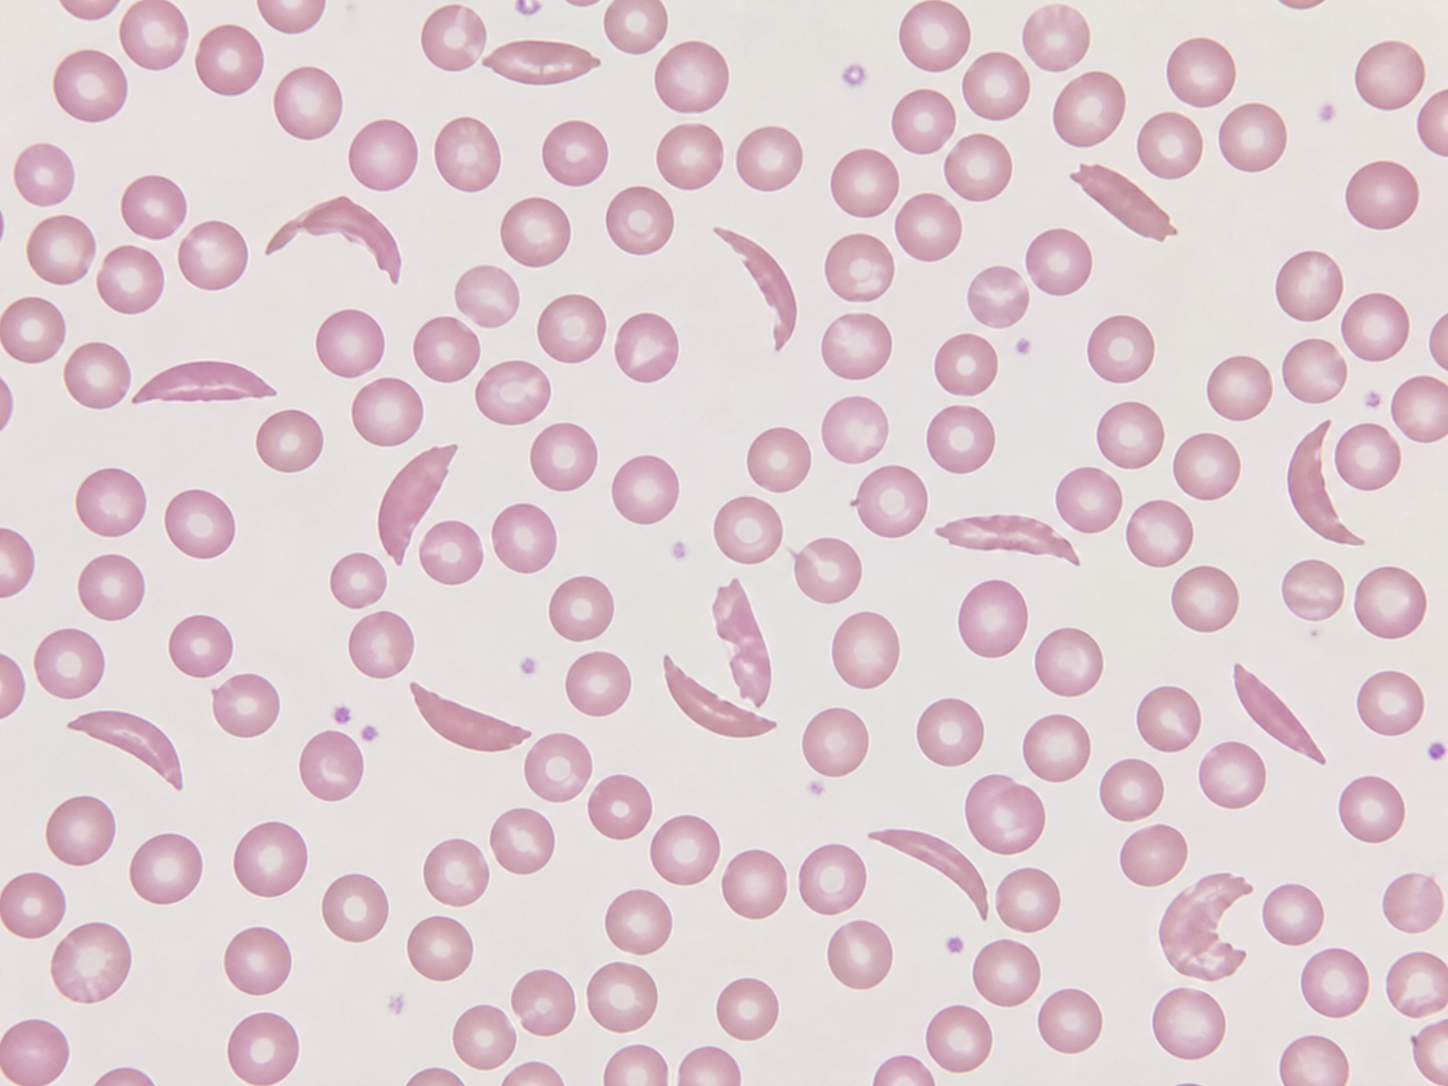
\includegraphics[width=0.56\linewidth]{images/book2/ai/g11-disease-sickle-smear.png}

{\small Apusan darah dari orang dengan penyakit \omterm{def:g10:cells-common-unit:cell}{sel} sabit: \omterm{def:g10:cells-common-unit:cell}{sel} merah
yang bulat dan, di antaranya, sabitnya. \omterm{def:g11:enzymes-and-phenotype:phenotype}{Fenotipe} seluler satu
substitusi \omterm{def:g10:chemistry-of-life:families}{asam amino}, yang terbawa pada kedua \omterm{def:g10:universal-dna:gene}{alelnya}.}
\end{omfigure}

\section{Membaca sebuah silsilah}

\begin{definition}[Silsilah]\label{def:g11:genes-and-disease:pedigree}
Sebuah \emph{silsilah}\index{silsilah} adalah bagan sebuah keluarga
sepanjang beberapa keturunan: persegi bagi lelaki, lingkaran bagi
perempuan, garis mendatar yang menghubungkan sepasang suami istri,
garis tegak turun ke anaknya, lambang terisi bagi orang yang terkena.
Keturunannya bernomor I, II, III dari atas; individunya bernomor dari kiri.
\end{definition}

\begin{omfigure}
\begin{tikzpicture}[font=\small, line cap=round]
  \tikzset{m/.style={draw, thick, minimum size=0.5cm, inner sep=0},
           f/.style={draw, thick, circle, minimum size=0.5cm, inner sep=0},
           aff/.style={fill=omThm!70}}
  % generation I
  \node[m] (I1) at (2,3) {}; \node[f] (I2) at (3.2,3) {};
  \node[m] (I3) at (6.4,3) {}; \node[f] (I4) at (7.6,3) {};
  \draw[thick] (I1) -- (I2); \draw[thick] (I3) -- (I4);
  \node[anchor=east] at (0.8,3) {I};
  \foreach \n/\x in {1/2, 2/3.2, 3/6.4, 4/7.6} \node[font=\scriptsize, anchor=south] at (\x,3.35) {\n};
  % generation II
  \draw[thick] (2.6,3) -- (2.6,2.3) -- (4.4,2.3); \draw[thick] (1.6,2.3) -- (2.6,2.3);
  \draw[thick] (7.0,3) -- (7.0,2.3) -- (5.6,2.3); \draw[thick] (7.0,2.3) -- (8.4,2.3);
  \node[f] (II1) at (1.6,1.7) {}; \node[m, aff] (II2) at (2.6,1.7) {}; \node[m] (II3) at (4.4,1.7) {};
  \node[f] (II4) at (5.6,1.7) {}; \node[f] (II5) at (7.0,1.7) {}; \node[m] (II6) at (8.4,1.7) {};
  \foreach \x in {1.6,2.6,4.4,5.6,7.0,8.4} \draw[thick] (\x,2.3) -- (\x,1.95);
  \draw[thick] (II3) -- (II4);
  \node[anchor=east] at (0.8,1.7) {II};
  \foreach \n/\x in {1/1.6, 2/2.6, 3/4.4, 4/5.6, 5/7.0, 6/8.4} \node[font=\scriptsize, anchor=north] at (\x,1.42) {\n};
  % generation III
  \draw[thick] (5.0,1.7) -- (5.0,1.0) -- (5.8,1.0); \draw[thick] (4.2,1.0) -- (5.0,1.0);
  \node[m] (III1) at (4.2,0.4) {}; \node[f, aff] (III2) at (5.8,0.4) {};
  \foreach \x in {4.2,5.8} \draw[thick] (\x,1.0) -- (\x,0.65);
  \node[anchor=east] at (0.8,0.4) {III};
  \foreach \n/\x in {1/4.2, 2/5.8} \node[font=\scriptsize, anchor=north] at (\x,0.12) {\n};
  % legend
  \node[m] at (10.2,2.6) {}; \node[anchor=west] at (10.5,2.6) {lelaki};
  \node[f] at (10.2,1.9) {}; \node[anchor=west] at (10.5,1.9) {perempuan};
  \node[m, aff] at (10.2,1.2) {}; \node[anchor=west] at (10.5,1.2) {terkena};
\end{tikzpicture}

{\small Sebuah \omterm{def:g11:genes-and-disease:pedigree}{silsilah} bagi fibrosis kistik. II-2 dan III-2 terkena;
orang tuanya sehat. Kedua pasangan I-1/I-2 dan II-3/II-4 pasti \omterm{def:g11:genes-and-disease:genetic}{pembawa};
II-3, saudara sehat seorang anak yang terkena, adalah \omterm{def:g11:genes-and-disease:genetic}{pembawa} dengan
peluang $2/3$.}
\end{omfigure}

\begin{method}[Menganalisis sebuah silsilah]\label{met:g11:genes-and-disease:analyse}
\begin{enumerate}
  \item \emph{\omterm{def:g11:genes-and-disease:genetic}{Dominan} atau \omterm{def:g11:genes-and-disease:genetic}{resesif}?} Anak yang terkena dari dua orang
        tua yang sehat berarti \omterm{def:g11:genes-and-disease:genetic}{resesif} (orang tuanya \omterm{def:g11:genes-and-disease:genetic}{pembawa}). Orang
        yang terkena dengan orang tua yang terkena pada tiap keturunan
        menyarankan \omterm{def:g11:genes-and-disease:genetic}{dominan}.
  \item \emph{Pada \omterm{def:g11:cell-cycle-mitosis:chromosome}{kromosom} kelamin?} Jika hanya lelaki yang terkena
        dan saudara lelaki ibunya atau ayahnya juga terkena, curigailah
        \omterm{def:g11:cell-cycle-mitosis:chromosome}{kromosom} X (di bawah). Jika tidak, \omterm{def:g10:universal-dna:gene}{gennya} ada pada \omterm{def:g11:cell-cycle-mitosis:chromosome}{kromosom}
        biasa.
  \item \emph{Tetapkan \omterm{def:g11:enzymes-and-phenotype:phenotype}{genotipenya}}: orang yang terkena pada penyakit
        \omterm{def:g11:genes-and-disease:genetic}{resesif} adalah $aa$; orang tua dan anaknya membawa sedikitnya
        satu $a$; saudara yang sehat dari orang yang terkena adalah
        $AA$ atau $Aa$.
  \item \emph{Hitunglah risikonya} bagi anak yang direncanakan dengan
        menggabungkan \omterm{def:g11:enzymes-and-phenotype:phenotype}{genotipe} orang tuanya dalam sebuah kotak Punnett;
        ketika \omterm{def:g11:enzymes-and-phenotype:phenotype}{genotipe} seorang tua tidak pasti, bobotilah tiap
        kemungkinannya dengan peluangnya.
\end{enumerate}
\end{method}

\begin{example}[Dua pertiganya]\label{ex:g11:genes-and-disease:twothirds}
Mengapa saudara lelaki yang sehat dari seorang anak yang terkena
menjadi \omterm{def:g11:genes-and-disease:genetic}{pembawa} dengan peluang $2/3$ dan bukan $1/2$? Orang tuanya
$Aa \times Aa$; seorang anak dapat berupa $AA$, $Aa$, $aA$ atau $aa$
dengan peluang yang sama. Mengetahui bahwa ia sehat menyingkirkan $aa$:
tiga hal tersisa, yang dua di antaranya \omterm{def:g11:genes-and-disease:genetic}{pembawa}. Jika ia menikahi
perempuan dari populasi umum (\omterm{def:g11:genes-and-disease:genetic}{pembawa} dengan peluang $1/25$), risiko
anak pertamanya terkena adalah $2/3 \times 1/25 \times 1/4 = 1/150$.
\end{example}

\section{Gen pada kromosom X}

\begin{proposition}[Pewarisan terpaut X]\label{prop:g11:genes-and-disease:xlinked}
Perempuan membawa dua \omterm{def:g11:cell-cycle-mitosis:chromosome}{kromosom} X, lelaki satu X dan satu Y. \omterm{def:g10:universal-dna:gene}{Alel}
\omterm{def:g11:genes-and-disease:genetic}{resesif} pada \omterm{def:g11:cell-cycle-mitosis:chromosome}{kromosom} X tertutupi pada perempuan oleh X keduanya,
tetapi lelaki, yang tidak punya X kedua, mengungkapkannya. Karena itu
penyakit semacam itu sebagian besar mengenai lelaki; anak perempuan
seorang lelaki yang terkena seluruhnya menjadi \omterm{def:g11:genes-and-disease:genetic}{pembawa}; seorang ibu
\omterm{def:g11:genes-and-disease:genetic}{pembawa} mewariskan \omterm{def:g10:universal-dna:gene}{alelnya} kepada separuh anak lelakinya, yang lalu
terkena, dan separuh anak perempuannya, yang lalu menjadi \omterm{def:g11:genes-and-disease:genetic}{pembawa}.
Hemofilia, yaitu darah yang gagal membeku, adalah contoh bakunya; buta
warna merah-hijau (\cref{ch:g11:the-eye}) adalah contoh yang lain.
\end{proposition}
\admitted

\begin{omfigure}
\begin{tikzpicture}[font=\small]
  \draw[thick] (0,0) grid[step=2.2] (4.4,4.4);
  \node[anchor=south] at (1.1,4.5) {$X^H$}; \node[anchor=south] at (3.3,4.5) {$Y$};
  \node[anchor=east] at (-0.15,3.3) {$X^H$}; \node[anchor=east] at (-0.15,1.1) {$X^h$};
  \node[anchor=south, font=\small\itshape] at (2.2,5.0) {ayah (sehat)};
  \node[font=\small\itshape, rotate=90, anchor=south] at (-0.95,2.2) {ibu (pembawa)};
  \node[fill=omDef!15, minimum size=2.1cm, align=center, font=\footnotesize] at (1.1,3.3) {$X^HX^H$\\ anak perempuan sehat};
  \node[fill=omDef!15, minimum size=2.1cm, align=center, font=\footnotesize] at (3.3,3.3) {$X^HY$\\ anak lelaki sehat};
  \node[fill=omProp!20, minimum size=2.1cm, align=center, font=\footnotesize] at (1.1,1.1) {$X^HX^h$\\ anak perempuan pembawa};
  \node[fill=omThm!25, minimum size=2.1cm, align=center, font=\footnotesize] at (3.3,1.1) {$X^hY$\\ anak lelaki terkena};
  \node[anchor=west, align=left, text width=6cm] at (5.4,2.2) {Ibu pembawa dan ayah yang sehat: separuh anak lelakinya terkena, separuh anak perempuannya menjadi pembawa, tidak ada anak perempuan yang terkena. $Y$ tidak membawa salinan gennya, sehingga satu-satunya salinan anak lelakinya berasal dari ibunya.};
\end{tikzpicture}

{\small Kotak Punnett bagi penyakit \omterm{def:g11:genes-and-disease:genetic}{resesif} terpaut X seperti hemofilia
($h$, \omterm{def:g10:universal-dna:gene}{alel} mutannya; $H$, \omterm{def:g10:universal-dna:gene}{alel} biasanya).}
\end{omfigure}

\section{Membaca gennya sendiri}

\begin{proposition}[Uji genetik]\label{prop:g11:genes-and-disease:testing}
\omterm{def:g10:universal-dna:gene}{Alel} yang dibawa seseorang dapat dibaca langsung dari \omterm{def:g10:universal-dna:information}{DNA-nya}, yang
disari dari beberapa \omterm{def:g10:cells-common-unit:cell}{sel} (darah, air liur, dan bagi janin sebuah
cuplikan plasenta atau cairan di sekelilingnya). Daerah \omterm{def:g10:universal-dna:gene}{gennya} disalin
jutaan kali oleh sebuah reaksi yang menirukan replikasi
(\cref{ch:g11:dna-replication}) dalam tabung reaksi, lalu urutannya
dibaca atau dipotong oleh \omterm{def:g11:enzymes-and-phenotype:enzyme}{enzim} yang mengenali urutan tertentu dan
dipilah menurut ukuran dalam sebuah gel: \omterm{def:g10:universal-dna:gene}{alel} mutan yang telah
memperoleh, kehilangan atau mengubah sebuah tapak potong memberi
penggalan dengan panjang yang berbeda, yang terlihat sebagai pita. Uji
semacam itu mengenali \omterm{def:g11:genes-and-disease:genetic}{pembawa} sebelum anak mana pun dikandung,
mendiagnosis janin, dan mengenali \omterm{def:g11:mutations:mutation}{mutasi} pada bayi baru lahir sebelum
gejalanya muncul.
\end{proposition}
\admitted

\begin{omfigure}
\begin{tikzpicture}[font=\small]
  % gel: 4 lanes
  \fill[gray!15] (0,0) rectangle (7.2,4.2);
  \foreach \x/\l in {0.9/{penanda\\ ukuran}, 2.7/{$AA$}, 4.5/{$Aa$}, 6.3/{$aa$}} \node[anchor=south, align=center] at (\x,4.3) {\l};
  % ladder
  \foreach \y in {3.6,3.1,2.6,2.0,1.4,0.8} \fill[omDef!70] (0.5,\y) rectangle (1.3,\y+0.1);
  % AA: one band (600 bp, cut into 400+200? keep: A allele = one long fragment at 3.1)
  \fill[omThm!80] (2.3,3.1) rectangle (3.1,3.2);
  % Aa: long fragment + two short
  \fill[omThm!80] (4.1,3.1) rectangle (4.9,3.2);
  \fill[omThm!80] (4.1,2.0) rectangle (4.9,2.1);
  \fill[omThm!80] (4.1,1.4) rectangle (4.9,1.5);
  % aa: two short only
  \fill[omThm!80] (5.9,2.0) rectangle (6.7,2.1);
  \fill[omThm!80] (5.9,1.4) rectangle (6.7,1.5);
  \draw[->, thick] (7.6,3.8) -- (7.6,0.8) node[midway, right, align=left] {arah\\ perpindahan:\\ penggalan kecil\\ berjalan lebih jauh};
  \node[anchor=east, font=\scriptsize] at (0.4,3.15) {600 bp};
  \node[anchor=east, font=\scriptsize] at (0.4,2.05) {400 bp};
  \node[anchor=east, font=\scriptsize] at (0.4,1.45) {200 bp};
\end{tikzpicture}

{\small Membaca \omterm{def:g10:universal-dna:gene}{alel} pada sebuah gel. \omterm{def:g10:universal-dna:gene}{Alel} mutan $a$ telah memperoleh
sebuah tapak potong: penggalan 600 pasangan \omterm{def:g10:universal-dna:nucleotide}{basa} milik $A$ terpotong
menjadi 400 dan 200. \omterm{def:g11:genes-and-disease:genetic}{Pembawa} memperlihatkan ketiga pitanya; orang yang
terkena hanya memperlihatkan kedua pita yang pendek.}
\end{omfigure}

\begin{omfigure}
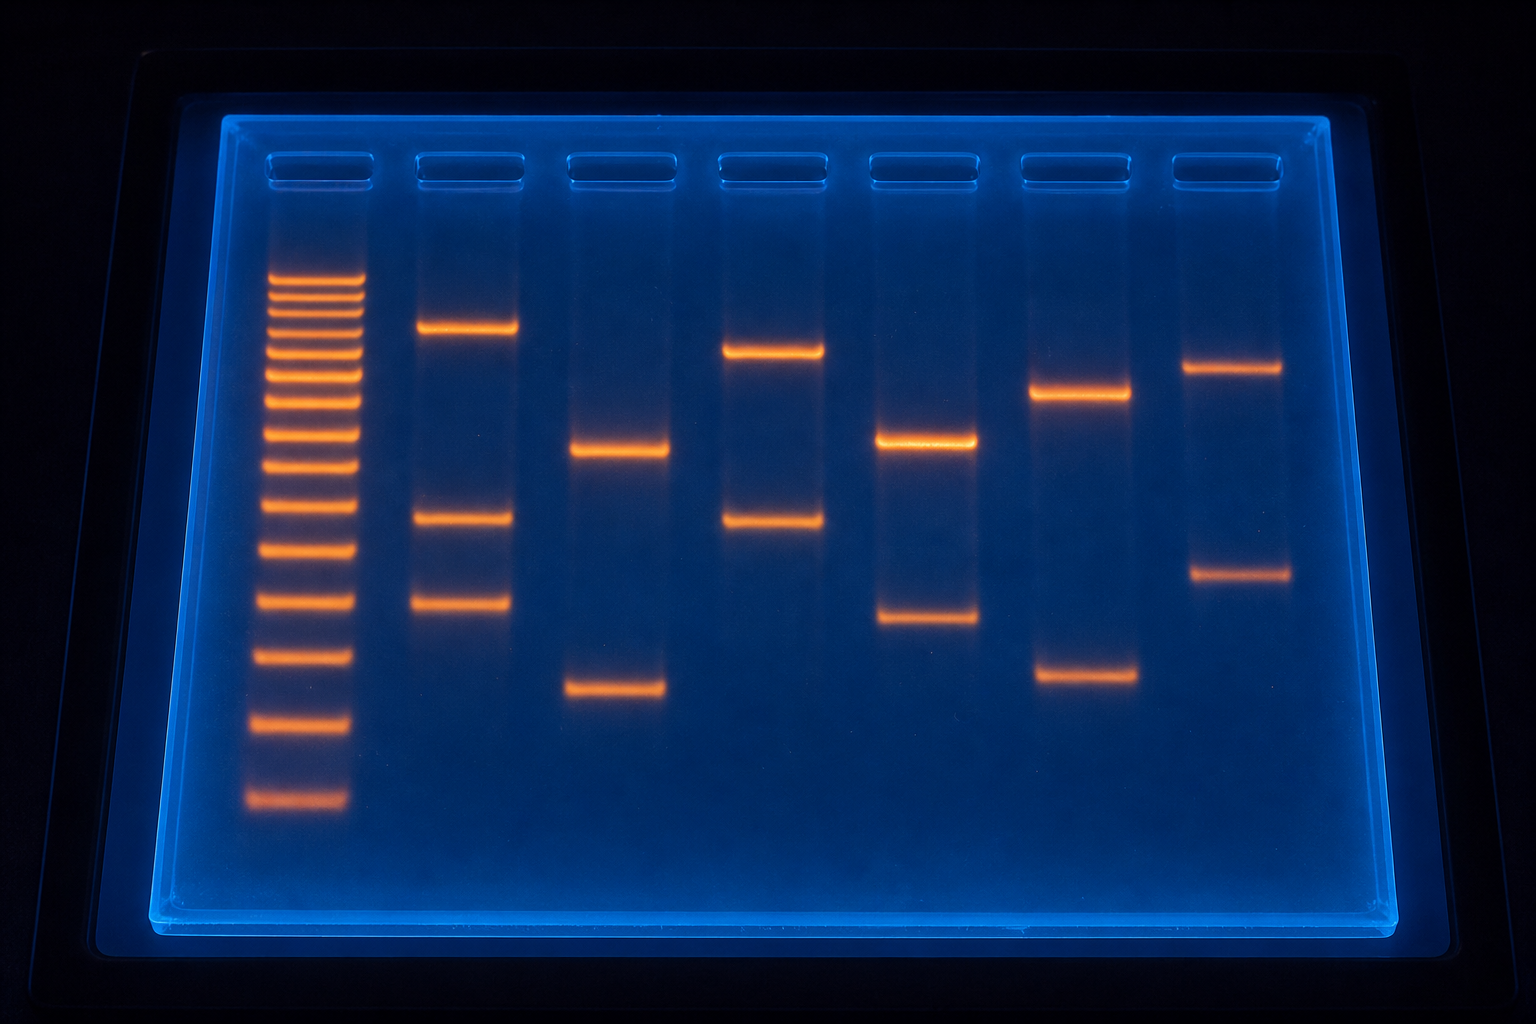
\includegraphics[width=0.56\linewidth]{images/book2/ai/g11-disease-gel.png}

{\small Sebuah gel elektroforesis di bawah cahaya ultraviolet:
penggalan \omterm{def:g10:universal-dna:information}{DNA}, yang diwarnai agar berpendar, terpilah menurut
panjangnya. Tiap lajurnya adalah satu cuplikan; pola pitanya membaca \omterm{def:g10:universal-dna:gene}{alelnya}.}
\end{omfigure}

\begin{example}[Apa yang dapat dan tidak dapat dinyatakan sebuah uji]\label{ex:g11:genes-and-disease:testsays}
Uji \omterm{def:g11:genes-and-disease:genetic}{pembawa} bagi fibrosis kistik mencari lima puluh \omterm{def:g10:universal-dna:gene}{alel} mutan yang
terlazim dan menemukan sekitar 90\% \omterm{def:g11:genes-and-disease:genetic}{pembawanya}: hasil yang negatif
menurunkan peluang seseorang menjadi \omterm{def:g11:genes-and-disease:genetic}{pembawa} dari $1/25$ menjadi
sekitar $1/250$, tetapi tidak membuatnya nol. Diagnosis pralahir pada
janin dari dua \omterm{def:g11:genes-and-disease:genetic}{pembawa} yang diketahui mendekati pasti, dan
menghadapkan orang tuanya pada keputusan yang tidak dibuatkan biologi
bagi mereka. Uji bagi penyakit Huntington memberi tahu seorang sehat
berumur tiga puluh apakah penyakitnya akan datang; sepertiga dari
mereka yang berhak atasnya memilih untuk tidak tahu.
\end{example}

\section{Penyakit banyak gen dan penyakit cara hidup}

\begin{proposition}[Penyakit multifaktor]\label{prop:g11:genes-and-disease:multifactorial}
Sebagian besar penyakit yang lazim --- diabetes tipe 2, penyakit
jantung dan arteri, sebagian besar kanker, asma --- bersifat
\emph{multifaktor}\index{penyakit multifaktor}: puluhan atau ratusan
\omterm{def:g10:universal-dna:gene}{alel} masing-masing menggeser risikonya sedikit, dan lingkungannya (pola
makan, kegiatan, merokok, infeksi) menggesernya banyak. Penyakit
semacam itu menurun dalam keluarga tanpa mengikuti aturan satu \omterm{def:g10:universal-dna:gene}{gen}, dan
kecenderungan genetik adalah sebuah risiko, bukan sebuah vonis: \omterm{def:g10:universal-dna:gene}{alel}
yang sama menghasilkan penyakit dalam satu cara hidup dan tidak dalam
cara hidup yang lain.
\end{proposition}
\begin{proof}[Bukti percobaan]
Kembar identik berbagi seluruh \omterm{def:g10:universal-dna:gene}{alelnya}; ketika yang satu mengidap
diabetes tipe 2, yang lain mengidapnya pada sekitar 70\% kasus --- jauh
di atas 8\% populasinya, sehingga \omterm{def:g10:universal-dna:gene}{gennya} menentukan --- tetapi bukan
100\%, sehingga \omterm{def:g10:universal-dna:gene}{gennya} tidak memutuskan. Populasi yang dalam satu
keturunan berpindah dari pola makan desa ke pola makan kota melihat
penyakitnya naik beberapa kali lipat dengan \omterm{def:g10:universal-dna:gene}{gen} yang sama. Di antara
orang yang membawa banyak \omterm{def:g10:universal-dna:gene}{alel} risiko, mereka yang tetap aktif dan
ramping mengidap penyakitnya dengan laju sepersekian laju mereka yang
tidak.
\end{proof}

\begin{omfigure}
\begin{tikzpicture}
\begin{axis}[
  ybar, bar width=12pt,
  width=0.8\linewidth, height=5.4cm,
  axis x line=bottom, axis y line=left,
  ymin=0, ymax=40, ylabel={diabetes tipe 2 sampai umur 60 (\%)},
  ylabel style={font=\small},
  symbolic x coords={sedikit alel risiko, rata-rata, banyak alel risiko},
  xtick=data, tick label style={font=\small},
  enlarge x limits=0.25, ytick={0,10,20,30,40},
  legend style={at={(0.5,-0.2)}, anchor=north, legend columns=2, font=\small, draw=none},
  nodes near coords, nodes near coords style={font=\scriptsize},
]
\addplot[fill=omMeth!50, draw=omMeth] coordinates {(sedikit alel risiko,3) (rata-rata,6) (banyak alel risiko,12)};
\addplot[fill=omThm!50, draw=omThm] coordinates {(sedikit alel risiko,9) (rata-rata,17) (banyak alel risiko,34)};
\legend{aktif dan ramping, kurang gerak dan kelebihan berat}
\end{axis}
\end{tikzpicture}

{\small Risiko diabetes tipe 2 menurut skor genetik dan cara hidupnya
(dibulatkan dari penelitian populasi). \omterm{def:g10:universal-dna:gene}{Gennya} melipatgandakan risikonya
empat kali dari satu ujung skalanya ke ujung yang lain; cara hidupnya
melipatgandakannya tiga kali pada tiap titik skalanya. Keduanya bekerja bersama.}
\end{omfigure}

\begin{remark}[Lalu apa arti ``genetik'']\label{rem:g11:genes-and-disease:meaning}
Fibrosis kistik bersifat genetik dalam arti yang ketat: \omterm{def:g11:enzymes-and-phenotype:phenotype}{genotipenya}
menetapkan penyakitnya, apa pun lingkungannya, dan lingkungannya hanya
mengubah cara penyakit itu dijalani. Diabetes tipe 2 bersifat genetik
dalam arti yang lebih lemah: \omterm{def:g11:enzymes-and-phenotype:phenotype}{genotipenya} menetapkan kerentanan yang
diwujudkan lingkungannya atau tidak. Di antara keduanya terletak
fenilketonuria, yang pola makannya membatalkan pengaruh \omterm{def:g11:enzymes-and-phenotype:phenotype}{genotipenya},
dan \omterm{def:g11:genes-and-disease:genetic}{pembawa} \omterm{def:g10:cells-common-unit:cell}{sel} sabit, yang \omterm{def:g10:universal-dna:gene}{alelnya} menjadi penyakit di satu tempat dan
perlindungan di tempat lain. ``Apakah ini genetik?'' jarang menjadi
pertanyaan ya-atau-tidak; ``seberapa besar, dan dalam keadaan apa?''
adalah pertanyaan yang patut diajukan.
\end{remark}

\section{Latihan}

\begin{exercise}[$\star$]\label{exo:g11:genes-and-disease:1}
Rumuskan \omterm{def:g10:universal-dna:gene}{alel} \omterm{def:g11:genes-and-disease:genetic}{resesif} dan \omterm{def:g10:universal-dna:gene}{alel} \omterm{def:g11:genes-and-disease:genetic}{dominan}, serta \omterm{def:g11:genes-and-disease:genetic}{pembawa}.
\end{exercise}

\begin{exercise}[$\star$]\label{exo:g11:genes-and-disease:2}
Dua \omterm{def:g11:genes-and-disease:genetic}{pembawa} fibrosis kistik punya seorang anak. Berikan peluang anaknya
terkena, menjadi \omterm{def:g11:genes-and-disease:genetic}{pembawa}, atau bukan keduanya.
\end{exercise}

\begin{exercise}[$\star$]\label{exo:g11:genes-and-disease:3}
Pada gambar \omterm{def:g11:genes-and-disease:pedigree}{silsilahnya}, berikan \omterm{def:g11:enzymes-and-phenotype:phenotype}{genotipe} I-1, I-2, II-2 dan
III-2.
\end{exercise}

\begin{exercise}[$\star$]\label{exo:g11:genes-and-disease:4}
Mengapa penyakit \omterm{def:g11:genes-and-disease:genetic}{resesif} terpaut X jauh lebih lazim pada lelaki?
\end{exercise}

\begin{exercise}[$\star$]\label{exo:g11:genes-and-disease:5}
Apa itu \omterm{prop:g11:genes-and-disease:multifactorial}{penyakit multifaktor}? Berikan dua contoh.
\end{exercise}

\begin{exercise}[$\star\star$]\label{exo:g11:genes-and-disease:6}
Seorang dengan fibrosis kistik menikahi seorang bukan \omterm{def:g11:genes-and-disease:genetic}{pembawa}.
Bagaimana anaknya? Dan bagaimana anak dari salah satu anaknya dengan
seorang \omterm{def:g11:genes-and-disease:genetic}{pembawa}?
\end{exercise}

\begin{exercise}[$\star\star$]\label{exo:g11:genes-and-disease:7}
Pada gambar \omterm{def:g11:genes-and-disease:pedigree}{silsilahnya}, hitung peluang II-1 menjadi \omterm{def:g11:genes-and-disease:genetic}{pembawa}, dan
peluang anak dari II-1 dan seorang lelaki dari populasi umum terkena.
\end{exercise}

\begin{exercise}[$\star\star$]\label{exo:g11:genes-and-disease:8}
Seorang lelaki dengan penyakit Huntington (\omterm{def:g11:genes-and-disease:genetic}{dominan}, satu \omterm{def:g10:universal-dna:gene}{alel} mutan)
dan seorang perempuan sehat punya empat anak. Berapa peluang seorang
anak tertentu mewarisi penyakitnya? Berapa peluang tidak satu pun dari
keempatnya mewarisinya?
\end{exercise}

\begin{exercise}[$\star\star$]\label{exo:g11:genes-and-disease:9}
Seorang lelaki hemofilia menikahi perempuan yang bukan \omterm{def:g11:genes-and-disease:genetic}{pembawa}.
Lukiskan \omterm{def:g11:enzymes-and-phenotype:phenotype}{genotipe} dan \omterm{def:g11:enzymes-and-phenotype:phenotype}{fenotipe} anaknya, dan \omterm{def:g11:enzymes-and-phenotype:phenotype}{genotipe} cucunya lewat
seorang anak perempuan yang menikah dengan lelaki yang sehat.
\end{exercise}

\begin{exercise}[$\star\star$]\label{exo:g11:genes-and-disease:10}
Pada gambar gelnya, pita apa yang akan diperlihatkan orang yang membawa
dua \omterm{def:g10:universal-dna:gene}{alel} mutan yang berbeda, satu yang menambahkan tapak potongnya dan
satu yang menghapus 100 pasangan \omterm{def:g10:universal-dna:nucleotide}{basa} lagi dari penggalan 400?
\end{exercise}

\begin{exercise}[$\star\star$]\label{exo:g11:genes-and-disease:11}
Jelaskan mengapa fibrosis kistik seribu kali lebih lazim di Eropa
daripada di Asia timur padahal laju \omterm{def:g11:mutations:mutation}{mutasinya} sama.
\end{exercise}

\begin{exercise}[$\star\star\star$]\label{exo:g11:genes-and-disease:12}
Anak pertama sepasang suami istri mengidap fibrosis kistik. Hitung
peluang anak kedua terkena, lalu peluang sedikitnya satu dari dua anak
berikutnya terkena. Jelaskan mengapa ``kami sudah mendapat satu dari
empatnya'' adalah kekeliruan.
\end{exercise}

\begin{exercise}[$\star\star\star$]\label{exo:g11:genes-and-disease:13}
Sebuah uji \omterm{def:g11:genes-and-disease:genetic}{pembawa} mengenali 90\% \omterm{def:g10:universal-dna:gene}{alel} mutannya. Seorang perempuan dari
populasi umum menerima hasil yang negatif. Hitung sisa peluangnya
menjadi \omterm{def:g11:genes-and-disease:genetic}{pembawa}, dan risiko anak yang terkena dengan pasangan yang
diketahui menjadi \omterm{def:g11:genes-and-disease:genetic}{pembawa}.
\end{exercise}

\begin{exercise}[$\star\star\star$]\label{exo:g11:genes-and-disease:14}
Dari gambar diabetesnya, bandingkan pengaruh berpindah dari ``banyak''
ke ``sedikit'' \omterm{def:g10:universal-dna:gene}{alel} risiko (mustahil) dengan pengaruh berpindah dari
kurang gerak ke aktif (mungkin), bagi orang dengan banyak \omterm{def:g10:universal-dna:gene}{alel} risiko.
Untuk apa sebaiknya skor risiko genetik dipakai?
\end{exercise}

\begin{exercise}[$\star\star\star$]\label{exo:g11:genes-and-disease:15}
Bahaslah, dalam satu paragraf, apa yang ditawarkan dan apa yang
dituntut uji penyakit Huntington dari seorang dewasa muda yang sehat
yang orang tuanya terkena, dan mengapa keputusannya ada padanya.
\end{exercise}

\section{Soal: Satu Keluarga, Satu Gen}

\begin{problem}[{Soal akhir pekan --- sebuah keluarga dengan fibrosis
kistik yang diikuti sepanjang tiga keturunan: genotipe yang ditetapkan,
risiko yang dihitung bagi tiap anak yang direncanakan, sebuah uji
laboratorium yang dibaca, dan hitungan sebuah populasi pembawa}]
\label{pb:g11:genes-and-disease:1}
Léa dan Tom, keduanya sehat, punya tiga anak: Max (sehat), Zoé
(fibrosis kistik) dan Lou (sehat). Ana, saudara perempuan Tom, sehat
dan menikah dengan Karim, yang keluarganya tidak punya riwayat
penyakitnya; keduanya sedang menantikan seorang anak. Dalam
populasinya, satu orang dari 25 adalah \omterm{def:g11:genes-and-disease:genetic}{pembawa}.

\medskip
\noindent\textbf{Bagian I --- \omterm{def:g11:enzymes-and-phenotype:phenotype}{Genotipenya}.}
\begin{enumerate}
  \item Apakah penyakitnya \omterm{def:g11:genes-and-disease:genetic}{dominan} atau \omterm{def:g11:genes-and-disease:genetic}{resesif}? Berikan alasannya dari
        keluarganya.
  \item Berikan \omterm{def:g11:enzymes-and-phenotype:phenotype}{genotipe} Léa, Tom dan Zoé.
  \item Apa saja \omterm{def:g11:enzymes-and-phenotype:phenotype}{genotipe} Max yang mungkin, dengan peluang berapa?
  \item Berapa peluang Ana menjadi \omterm{def:g11:genes-and-disease:genetic}{pembawa}? (Tinjaulah orang tuanya.)
  \item Berapa peluang Karim menjadi \omterm{def:g11:genes-and-disease:genetic}{pembawa}?
\end{enumerate}

\medskip
\noindent\textbf{Bagian II --- Risikonya.}
\begin{enumerate}[resume]
  \item Hitung peluang anak Ana dan Karim terkena.
  \item Léa dan Tom mempertimbangkan anak keempat. Berapa peluangnya
        terkena? Berapa peluangnya menjadi \omterm{def:g11:genes-and-disease:genetic}{pembawa}?
  \item Max, setelah dewasa, menikahi perempuan dari populasi umum.
        Berapa peluang anak pertamanya terkena?
  \item Zoé, setelah dewasa, menikahi lelaki dari populasi umum.
        Berapa peluang anaknya terkena? Berapa peluang anaknya menjadi
        \omterm{def:g11:genes-and-disease:genetic}{pembawa}?
  \item Lou menikahi sepupu pertamanya, yaitu anak Ana dan Karim.
        Hitung peluang anaknya terkena. Mengapa peluangnya lebih tinggi
        daripada peluang Max?
\end{enumerate}

\medskip
\noindent\textbf{Bagian III --- Ujinya.}
\omterm{def:g10:universal-dna:gene}{Alel} mutan yang dibawa keluarga ini menambahkan sebuah tapak potong:
\omterm{def:g10:universal-dna:gene}{alel} biasanya memberi satu penggalan 900 pasangan \omterm{def:g10:universal-dna:nucleotide}{basa}, \omterm{def:g10:universal-dna:gene}{alel} mutannya
memberi 600 dan 300.
\begin{enumerate}[resume]
  \item Gambarkan, atau lukiskan, pita yang diharapkan bagi Zoé, bagi
        Tom, dan bagi seorang bukan \omterm{def:g11:genes-and-disease:genetic}{pembawa}.
  \item Max diuji: satu pita pada 900. Apa \omterm{def:g11:enzymes-and-phenotype:phenotype}{genotipenya} sekarang, dan
        berapa risiko baru bagi anak pertamanya (pertanyaan 8)?
  \item Ana diuji: pita pada 900, 600 dan 300. Hitung ulang risiko bagi
        anaknya.
  \item Uji Karim tidak menemukan satu pun dari lima puluh \omterm{def:g10:universal-dna:gene}{alel} mutan
        yang terlazim, yang meliput 90\% \omterm{def:g11:genes-and-disease:genetic}{pembawanya}. Hitung sisa
        peluangnya menjadi \omterm{def:g11:genes-and-disease:genetic}{pembawa} lalu hitung ulang risikonya.
  \item Uji pralahir pada janin Ana dan Karim memperlihatkan pita pada
        900, 600 dan 300. Apa \omterm{def:g11:enzymes-and-phenotype:phenotype}{genotipe} dan \omterm{def:g11:enzymes-and-phenotype:phenotype}{fenotipe} janinnya?
\end{enumerate}

\medskip
\noindent\textbf{Bagian IV --- Populasinya.}
\begin{enumerate}[resume]
  \item Jika satu orang dari 25 adalah \omterm{def:g11:genes-and-disease:genetic}{pembawa}, berapa peluang kedua
        anggota sepasang suami istri acak menjadi \omterm{def:g11:genes-and-disease:genetic}{pembawa}, dan dengan
        demikian berapa frekuensi bayi baru lahir yang terkena?
  \item Bandingkan dengan satu dari 2500 yang teramati. Beri tanggapan.
  \item Dahulu hampir seluruh orang yang terkena meninggal pada masa
        kanak-kanak. Jelaskan mengapa \omterm{def:g10:universal-dna:gene}{alel} mutannya tetap bertahan pada
        frekuensi satu dari 50 salinan, dengan memakai jumlah salinan
        yang dibawa \omterm{def:g11:genes-and-disease:genetic}{pembawa} yang sehat dibandingkan dengan yang dibawa
        orang yang terkena.
  \item Pengobatan kini membiarkan sebagian besar orang yang terkena
        mencapai usia dewasa dan punya anak. Ramalkan pengaruhnya pada
        frekuensi \omterm{def:g10:universal-dna:gene}{alelnya} sepanjang keturunan mendatang, dan besarnya.
  \item Nyatakan hasilnya: satu-dari-empat bagi dua \omterm{def:g11:genes-and-disease:genetic}{pembawa},
        dua-dari-tiga bagi saudara yang sehat, dan apa yang ditambahkan
        gelnya pada hitungan keluarga ini.
\end{enumerate}
\end{problem}
